\documentclass[a4paper,12pt]{article}

\usepackage{color}
\usepackage{graphicx}
\usepackage[parfill]{parskip}	% skip a line instead of no indent on first line
\usepackage{natbib}			% lets you cite name and/or year instead of number

\begin{document}
\title{My First Document}
\author{Ronan Connolly}
\date{\today}
\maketitle

\pagenumbering{roman}
\tableofcontents
\newpage
\pagenumbering{arabic}

\section{Introduction}
This is the introduction.

\section{Methods}

\subsection{Stage 1}
\label{sec1}
The first part of the methods.

\subsection{Stage 2}
The second part of the methods.

\section{Results}
Here are my results. Referring to section \ref{sec1} on page \pageref{sec1}.

\section{Typesetting Text}
\subsection{font effects}

\textit{words in italics}
\textsl{slanted words}
\textsc{All These Words are in Small Caps}
\textbf{bold words}
\texttt{Words in teletype}
\textsf{Words in sans serif}
\textrm{Roman words}
\underline{underlined words}

\subsection{coloured text}
{\color{cyan}I am cyan!}
{\color{red} fire.}

\subsection{font sizes}
{\tiny tiny words}
{\scriptsize scriptsize words}
{\footnotesize footnotesize words}
{\small small words}
{\normalsize normalsize words}
{\large large words}
{\Large Large words}
{\huge huge words}

\subsection{lists}
\begin{enumerate}
\item[-] First thang first
\item[+] Second thing
\begin{itemize}
\item[fish] A sub-thang
\item[Plants] another sub-thang
\end{itemize}
\item Third thing
\end{enumerate}

\subsection{comments \& spacing}
It is a truth universally acknowledged % Note comic irony in the first sentence
, that a single man in possession of a good fortune, must be in want of a wife.

Line 1


Line 2






Line 3
Line 4
\\

New line
\\

Another new line
same line

new paragraph

I woud like some vertical space below \vspace{102pt}

102pt above?

\subsection{special characters}

backslash: \textbackslash

\# \$ \% \^{} \& \_ \{ \} \~{}

\^ e
\~ e

\textbf {Text Test}
\\
Item \#1A\textbackslash642 costs \$8 \& is sold at a \~{}10\% profit.

\section{Tables}
\begin{tabular}{|l|l|}
Apples & Green \\
Stawberries & Red \\
Oranges & Oranges \\
\end{tabular}

\begin{tabular}{rc}
Apples & Green \\
\hline
Stawberries & Red \\
\cline{1-1}
Oranges & Oranges \\
\end{tabular}

\begin{tabular}{|r|l|}
\hline
8 & here's \\
\cline{2-2}
68 & stuff \\
\hline \hline
2008 & now \\
\hline
\end{tabular}


\subsection{practical}
\begin{tabular}{l|r|r}
Item & Quantity & Price (\$) \\
\hline
Nail & 500 & 0.34 \\
Wooden boards & 100 & 4.00 \\
Bricks & 240 & 11.50 \\
\end{tabular}
\\
\\

\begin{tabular}{l|ccc}
&&Year \\
\cline{2-4}
City & 2006 & 2007 & 2008 \\
\hline
London & 45789 & 45345 & 87654 \\
Berlin & 45789 & 45345 & 87654 \\
Paris & 45789 & 45345 & 87654 \\
\end{tabular}

\newpage

\section{Figures}
\textbf{Inserting images!}

\begin{figure}[h]
\centering
%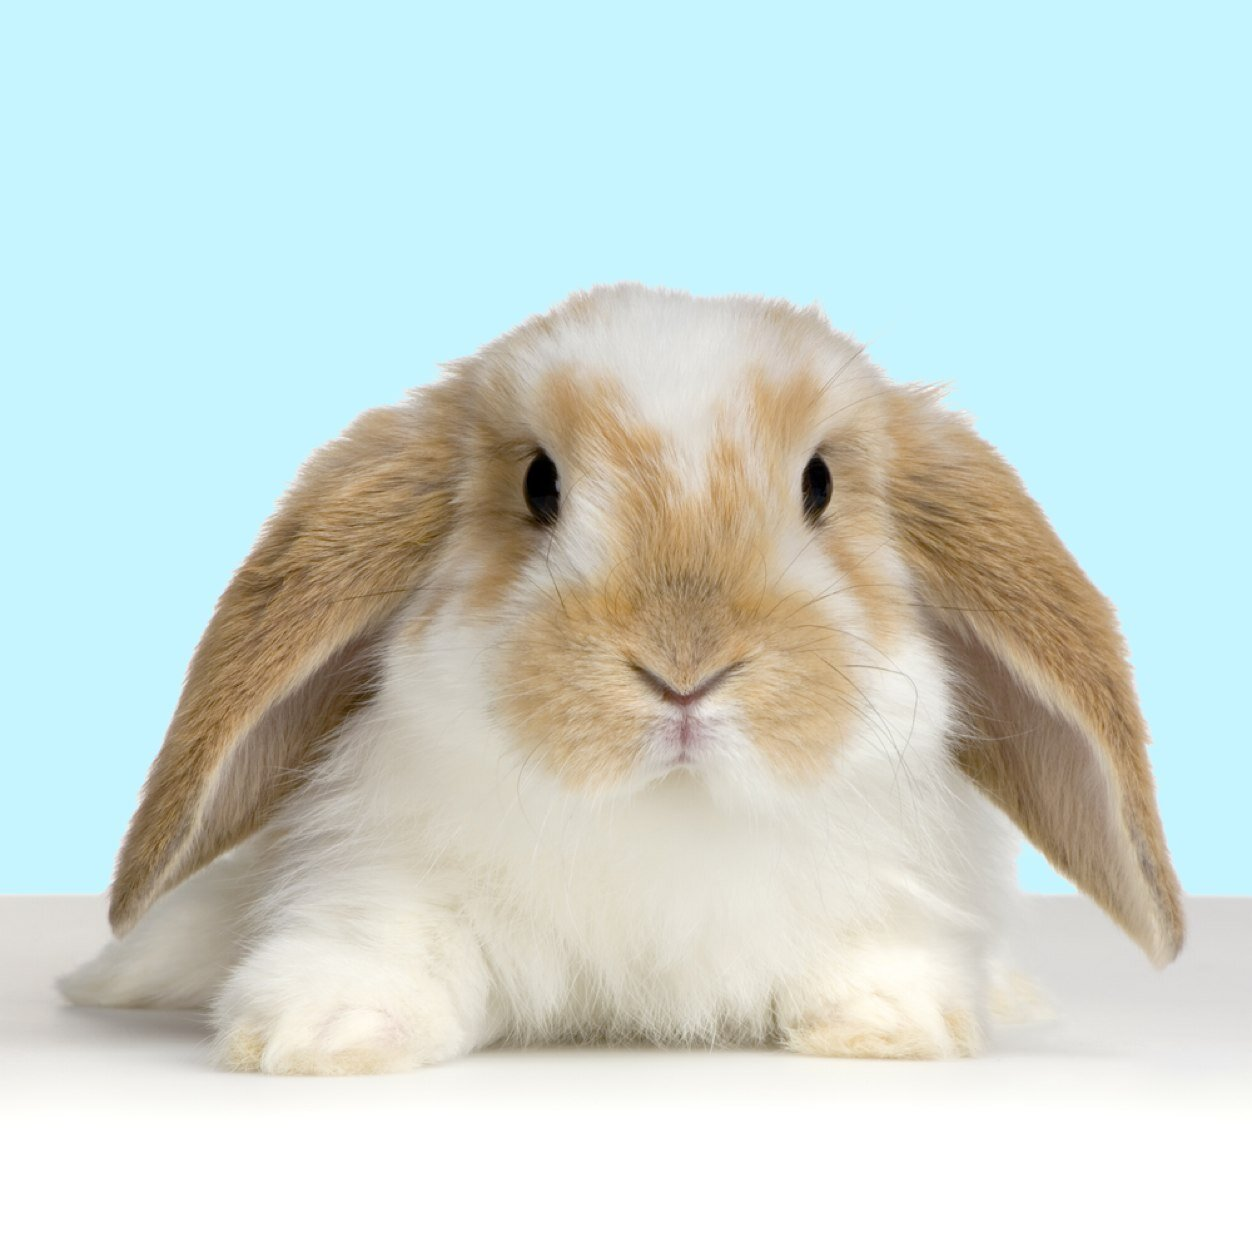
\includegraphics[width=1\textwidth]{myimage}
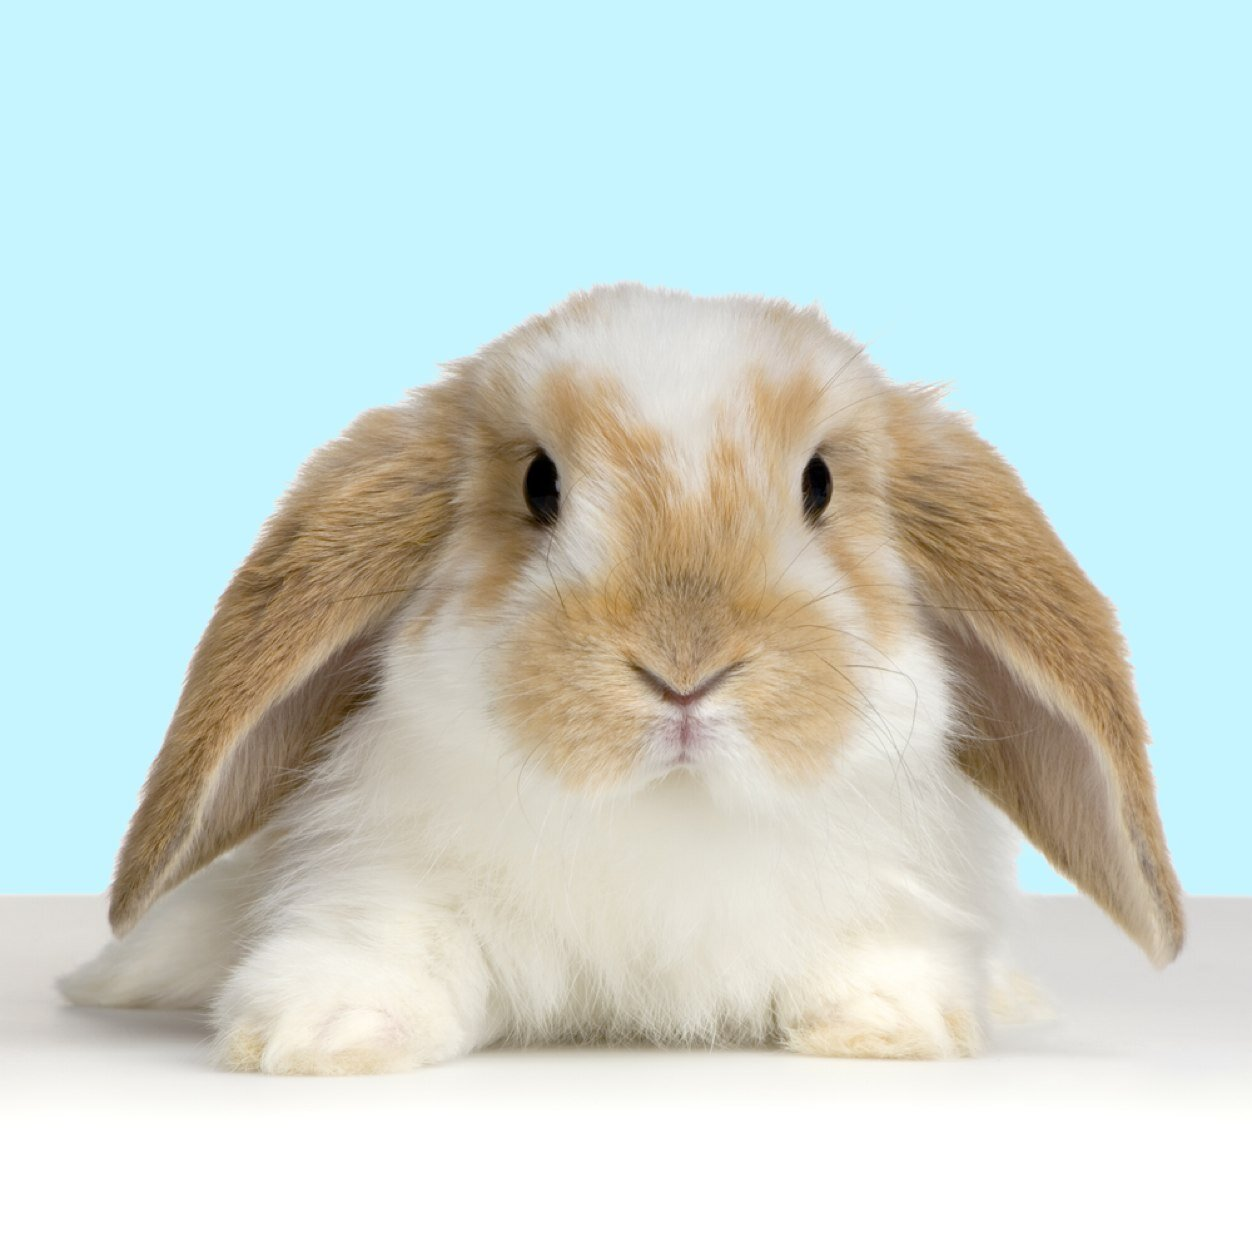
\includegraphics[scale=0.2]{myimage}
\caption{A bunny}
\label{image-myimage}
\end{figure}

\begin{figure}[h!]
\centering
\includegraphics[width=0.5\textwidth]{"myimage"}
\caption{My test image, another bunny}
\end{figure}


\section{Equations}
\subsection{inserting equations}
$Math mode$

$1+2=3$

%display equation on own line
$$1+2=3$$

%numbered displayed equation
\begin{equation}
1+2=3
\end{equation}

% (*=unumbered) series of equations
\begin{eqnarray*}
a & = & b + c \\
   & = & y - z
\end{eqnarray*}


\newpage
\newpage

\subsection{Mathamatical Symbols}
\subsubsection{Powers \& Indices}

Maths:
\\

Power:     
$n^2$

Indice: 
$2_a$

Symbol uses more than one character? 
$b_{a-2}$

\subsubsection{Fractions}
numerator then 
denominator
$$\frac{a}{3}$$

Nested:
$$\frac{y}{\frac{3}{x}+b}$$

\subsubsection{Roots}
Square Root:
$$\sqrt{y^2}$$
$$\sqrt[x]{y^2}$$


\subsubsection{Sums \& Integral}
Title:

Sum:
$$\sum$$
$$\sum_{x=1}^5 y^z$$

Integral:
$$\int$$
$$\int_a^b f(x)$$


\subsubsection{Greek Letters}
title

alpha:
$\alpha$

beta:
$\beta$

delta:
$\delta, \Delta$

theta:
$\theta, \Theta$

mu:
$\mu$

pi:
$\pi, \Pi$

sigma:
$\sigma, \Sigma$

phi:
$\phi, \Phi$

psi:
$\psi, \Psi$

omega:
$\omega, \Omega$


\subsubsection{Practical}
\begin{eqnarray}
e = mc^2 \\
\pi = \frac{c}{d} \\
\frac{d}{dx}e^x = e^x \\
\frac{d}{dx}\int_0^\infty f(s)ds = f(x) \\
f(x) = \sum_i = 0^\infty\frac{f^(i)(0)}{i!}x^i \\
x = \sqrt{\frac{x_i}{z}y}
\end{eqnarray}


\section{Referencing}
\subsection{BibText File}
Created.
$$Doc1.bib$$

\subsection{Inserting the bibliography}
cite:
\cite{Connollyetal2014}

nocite:
\nocite{Connollyetal2016}

page number:
\cite[p.214]{Connollyetal2016}

site multiple:
\cite{Connollyetal2016, Connollyetal2015, Connollyetal2014, Connollyetal2013}

\subsection{Citing References}

\subsection{Styles}
\subsubsection{Numerical Citations}
Plain:

The bibliography is ordered alphabetically by first author surname

\subsubsection{Author-date citations}
natbib package

include author-date citations:
\citep{Connollyetal2016}

Only year in brackets
\citet{Connollyetal2016}

\subsubsection{Other bibliography styles}
In order to use external style files then save the style fil (.bst) in the same folder as the .tex and .bib of project.

Include the bst file name in:
\begin{verbatim}
\bibliographystyle{...}
\end{verbatim}


\subsection{practical}

\section{Further Reading}
We need some emoji tags, it's $2k16!$

{\huge \color{cyan}{\LaTeX}}

\section{test}

\begin{verbatim}
\it This is how you write in italic
\end{verbatim}

\bibliography{Doc1}{}
\bibliographystyle{plain}
%\bibliographystyle{abbrv}
%\bibliographystyle{unsrt}
%\bibliographystyle{alpha}
%\bibliographystyle{plainnat}


\end{document}